
As mention in the use cases for the application, all of the application's functionality should be accessible by using gestures. The user should thus
be able to do every task only by using gestures (except looking around, which can only be done by rotating the HMD). To support this a gesture scheme of seven (or eight depending
on perspective) individual gestures were created. The gestures can all be considered static gestures, meaning that they don't require movement for the gesture to be detected, 
except for the movement required to form the gesture. 
Even though the gestures can be considered static in this aspect, the user is still often required to move his or her hand while holding the gesture to get the desired effect. 
The application should also give visual feedback when a gesture is recognized. This could be by altering the hand model in some way (e.g~color it differently by
switching materials) or by having some user interface showing it. 


The gestures are individually described below on a functional level and will be covered in more technical detail during the our review of the implementation in chapter~\ref{chapter:implementation}. 
Both the left- and right hand should be able to execute all these gestures independently, so scenarios where both hands do the same gestures, or different gestures, should
work. The only exception from this is the menu gesture, where one hand is assigned to be "the menu hand" (the left hand by default) and one is assigned to be "the selector hand"
(right by default). The gestures are designed to be as distinguishable from each other as possible to decrease the possibility of one gesture being mistaken for another
by the gesture recognition system. The gestures should also be distinguishable from different angles, and thus support different camera positions (assuming a vision-based system).


\subsection{The Pinch Gesture}
The pinch gesture will enable the user to rotate - and thus change orientation- by the Y and Z axis, as specified in "rotate-use case". 
The pinch gesture is accomplished by squeezing the tip of the thumb and index fingers together while, preferably, keeping the rest of the fingers erect and the palm facing 
somewhere between the table top and the displays (see~\vref{fig:gestures1} for an illustration). Once this gesture is done by the user, 
the system should indicate that the gesture was recognized as a pinch gesture.
Once the system has recognized the pinch gesture it should store the x, y and z coordinates - the position where the gesture was first detected - as an origin point and start rotating the 
camera with the offset value of this origin point. This means that when the user perform a pinch gesture without moving the hand, the pinch gesture should be detected and be
"active", but the camera should not be moved. If the user then moves his or her hand to the right, while still keeping the pinch gesture, the camera should start rotating 
to the right also. If the user moves his or her hand further to the right the camera should start rotate at a faster rate than previously.  
The primary idea behind this origin-offset scheme, which also are used in other gestures, is to prevent user fatigue by allowing the user to execute
the gesture in the position that feels most comfortable, as long as this position is captured by the vision-based gesture recognition system. 
In addition this scheme also prevents the user from having to move his or her hands as much as some other schemes would (e.g.~dragging motions).  

\begin{figure}%[h!] %[H]
	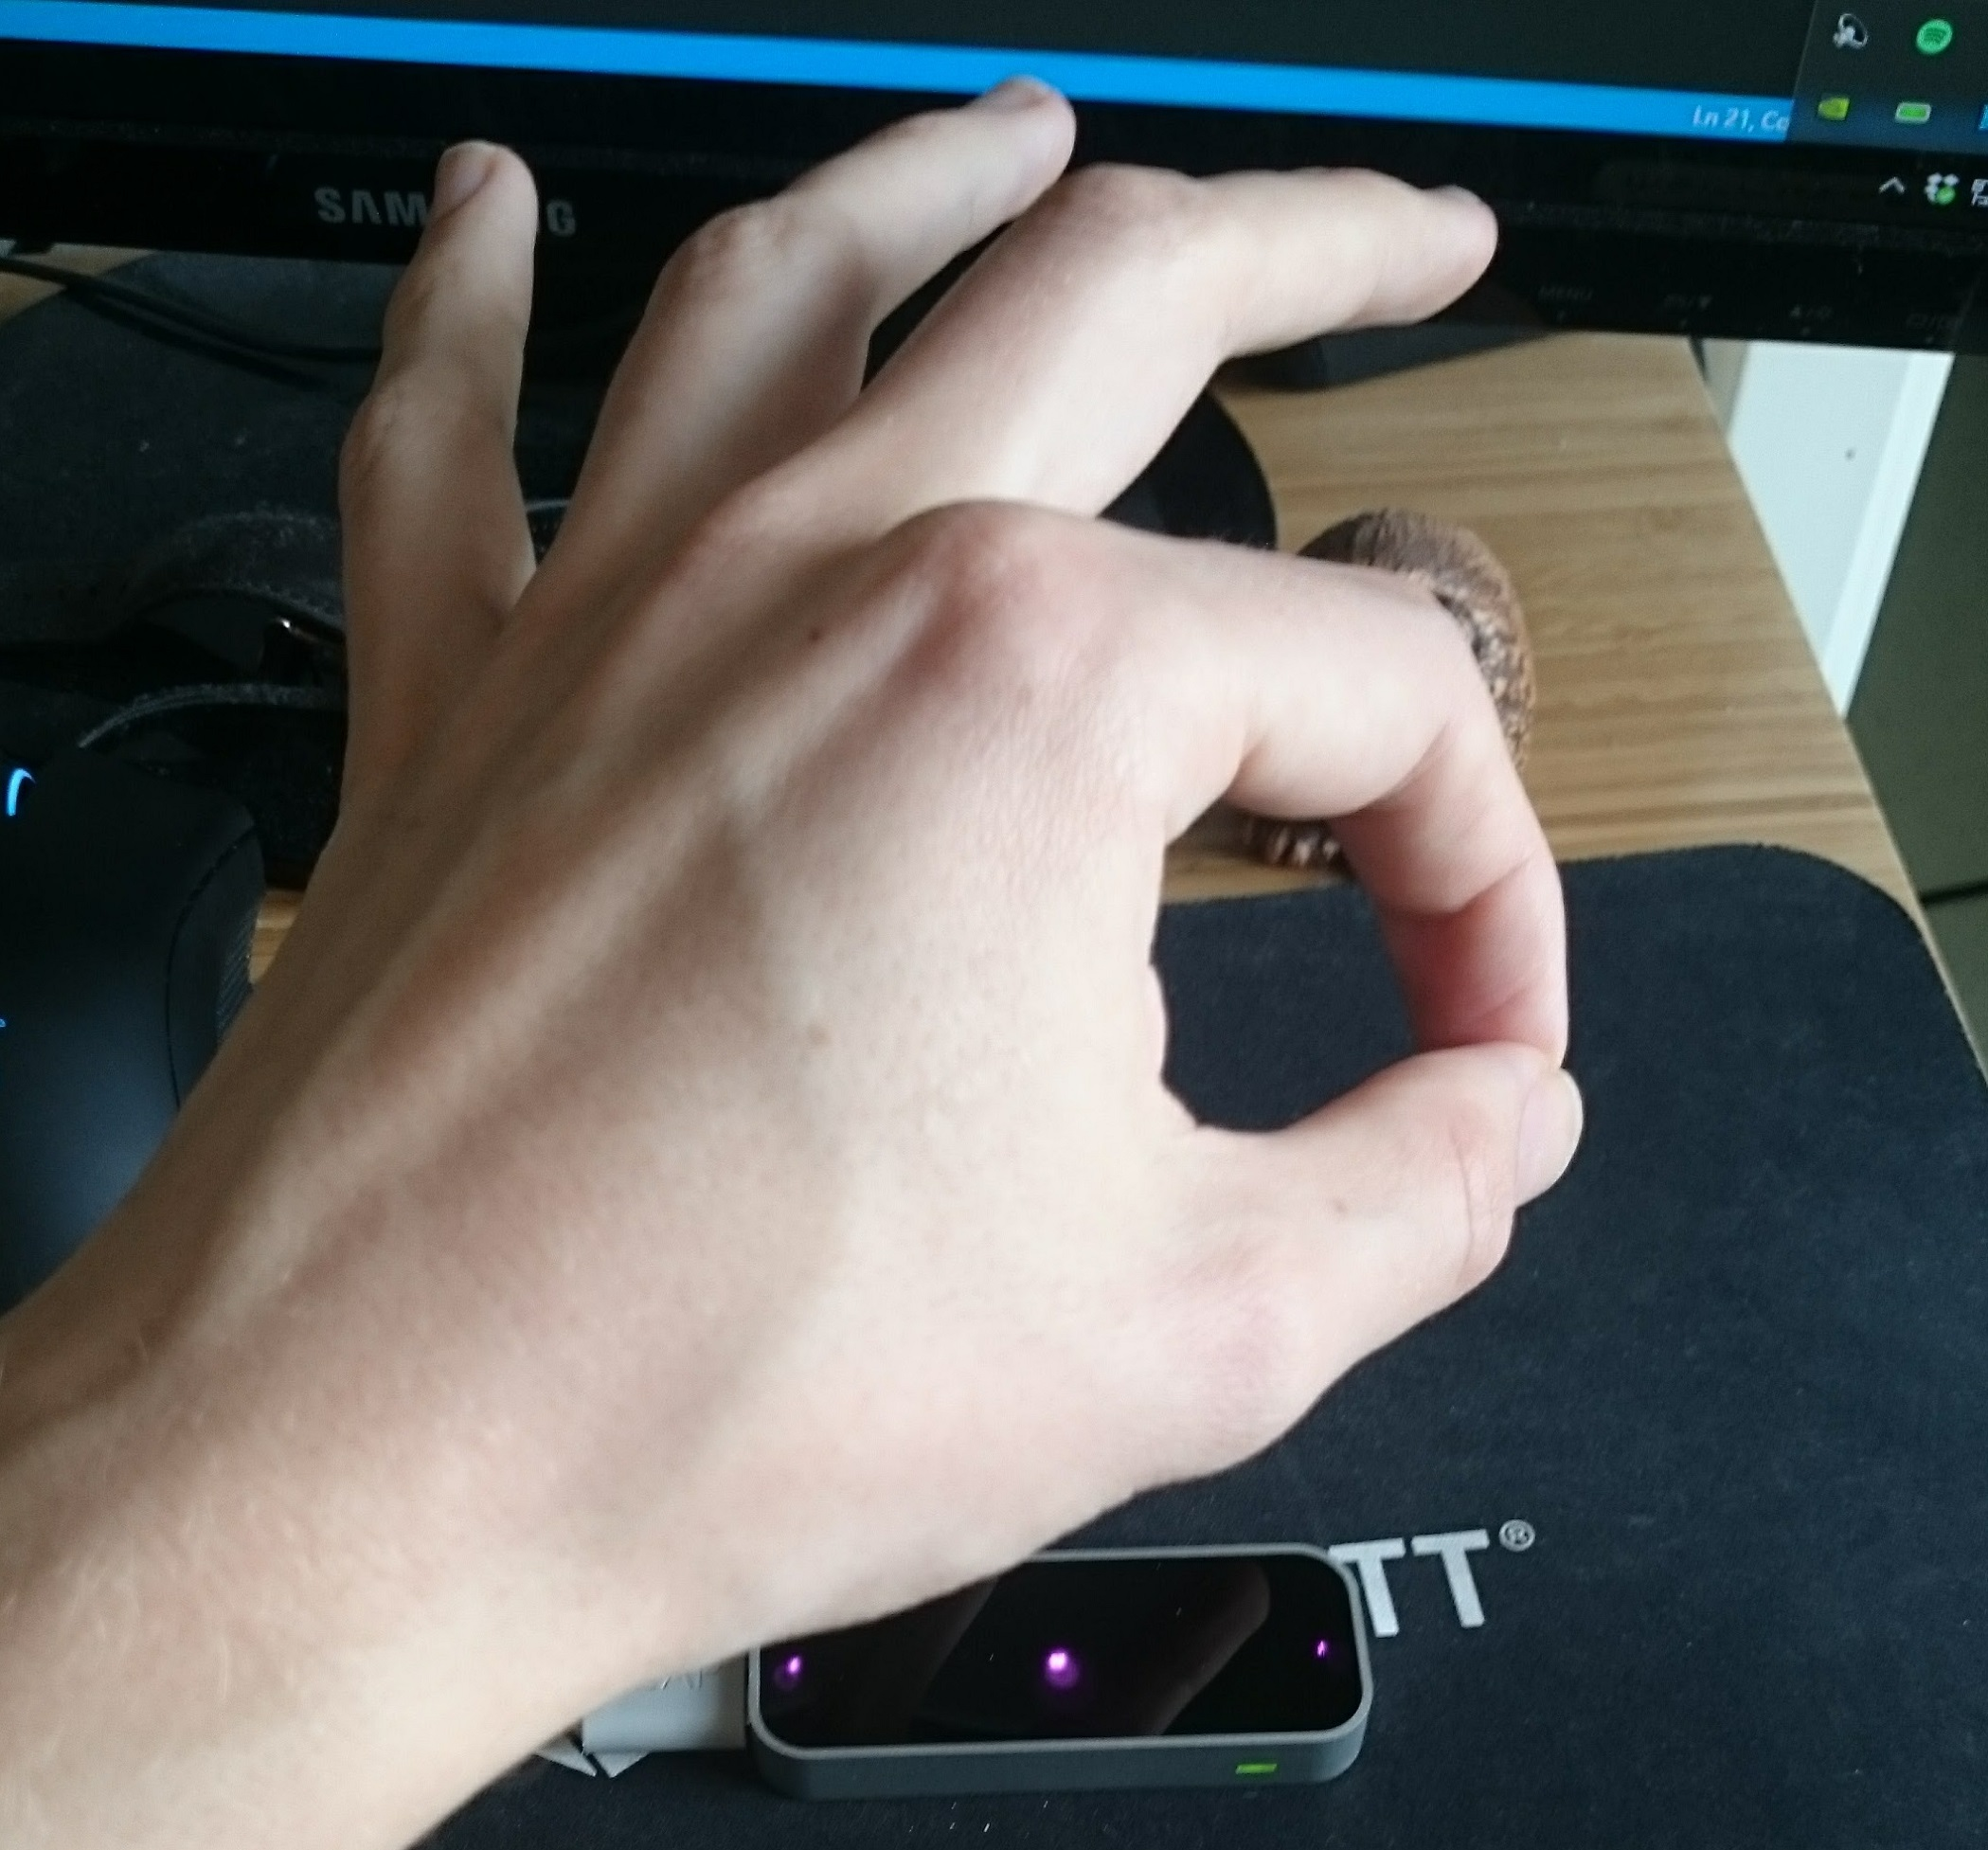
\includegraphics[width=0.5\linewidth]{pictures/gestures/pinch.jpg}
    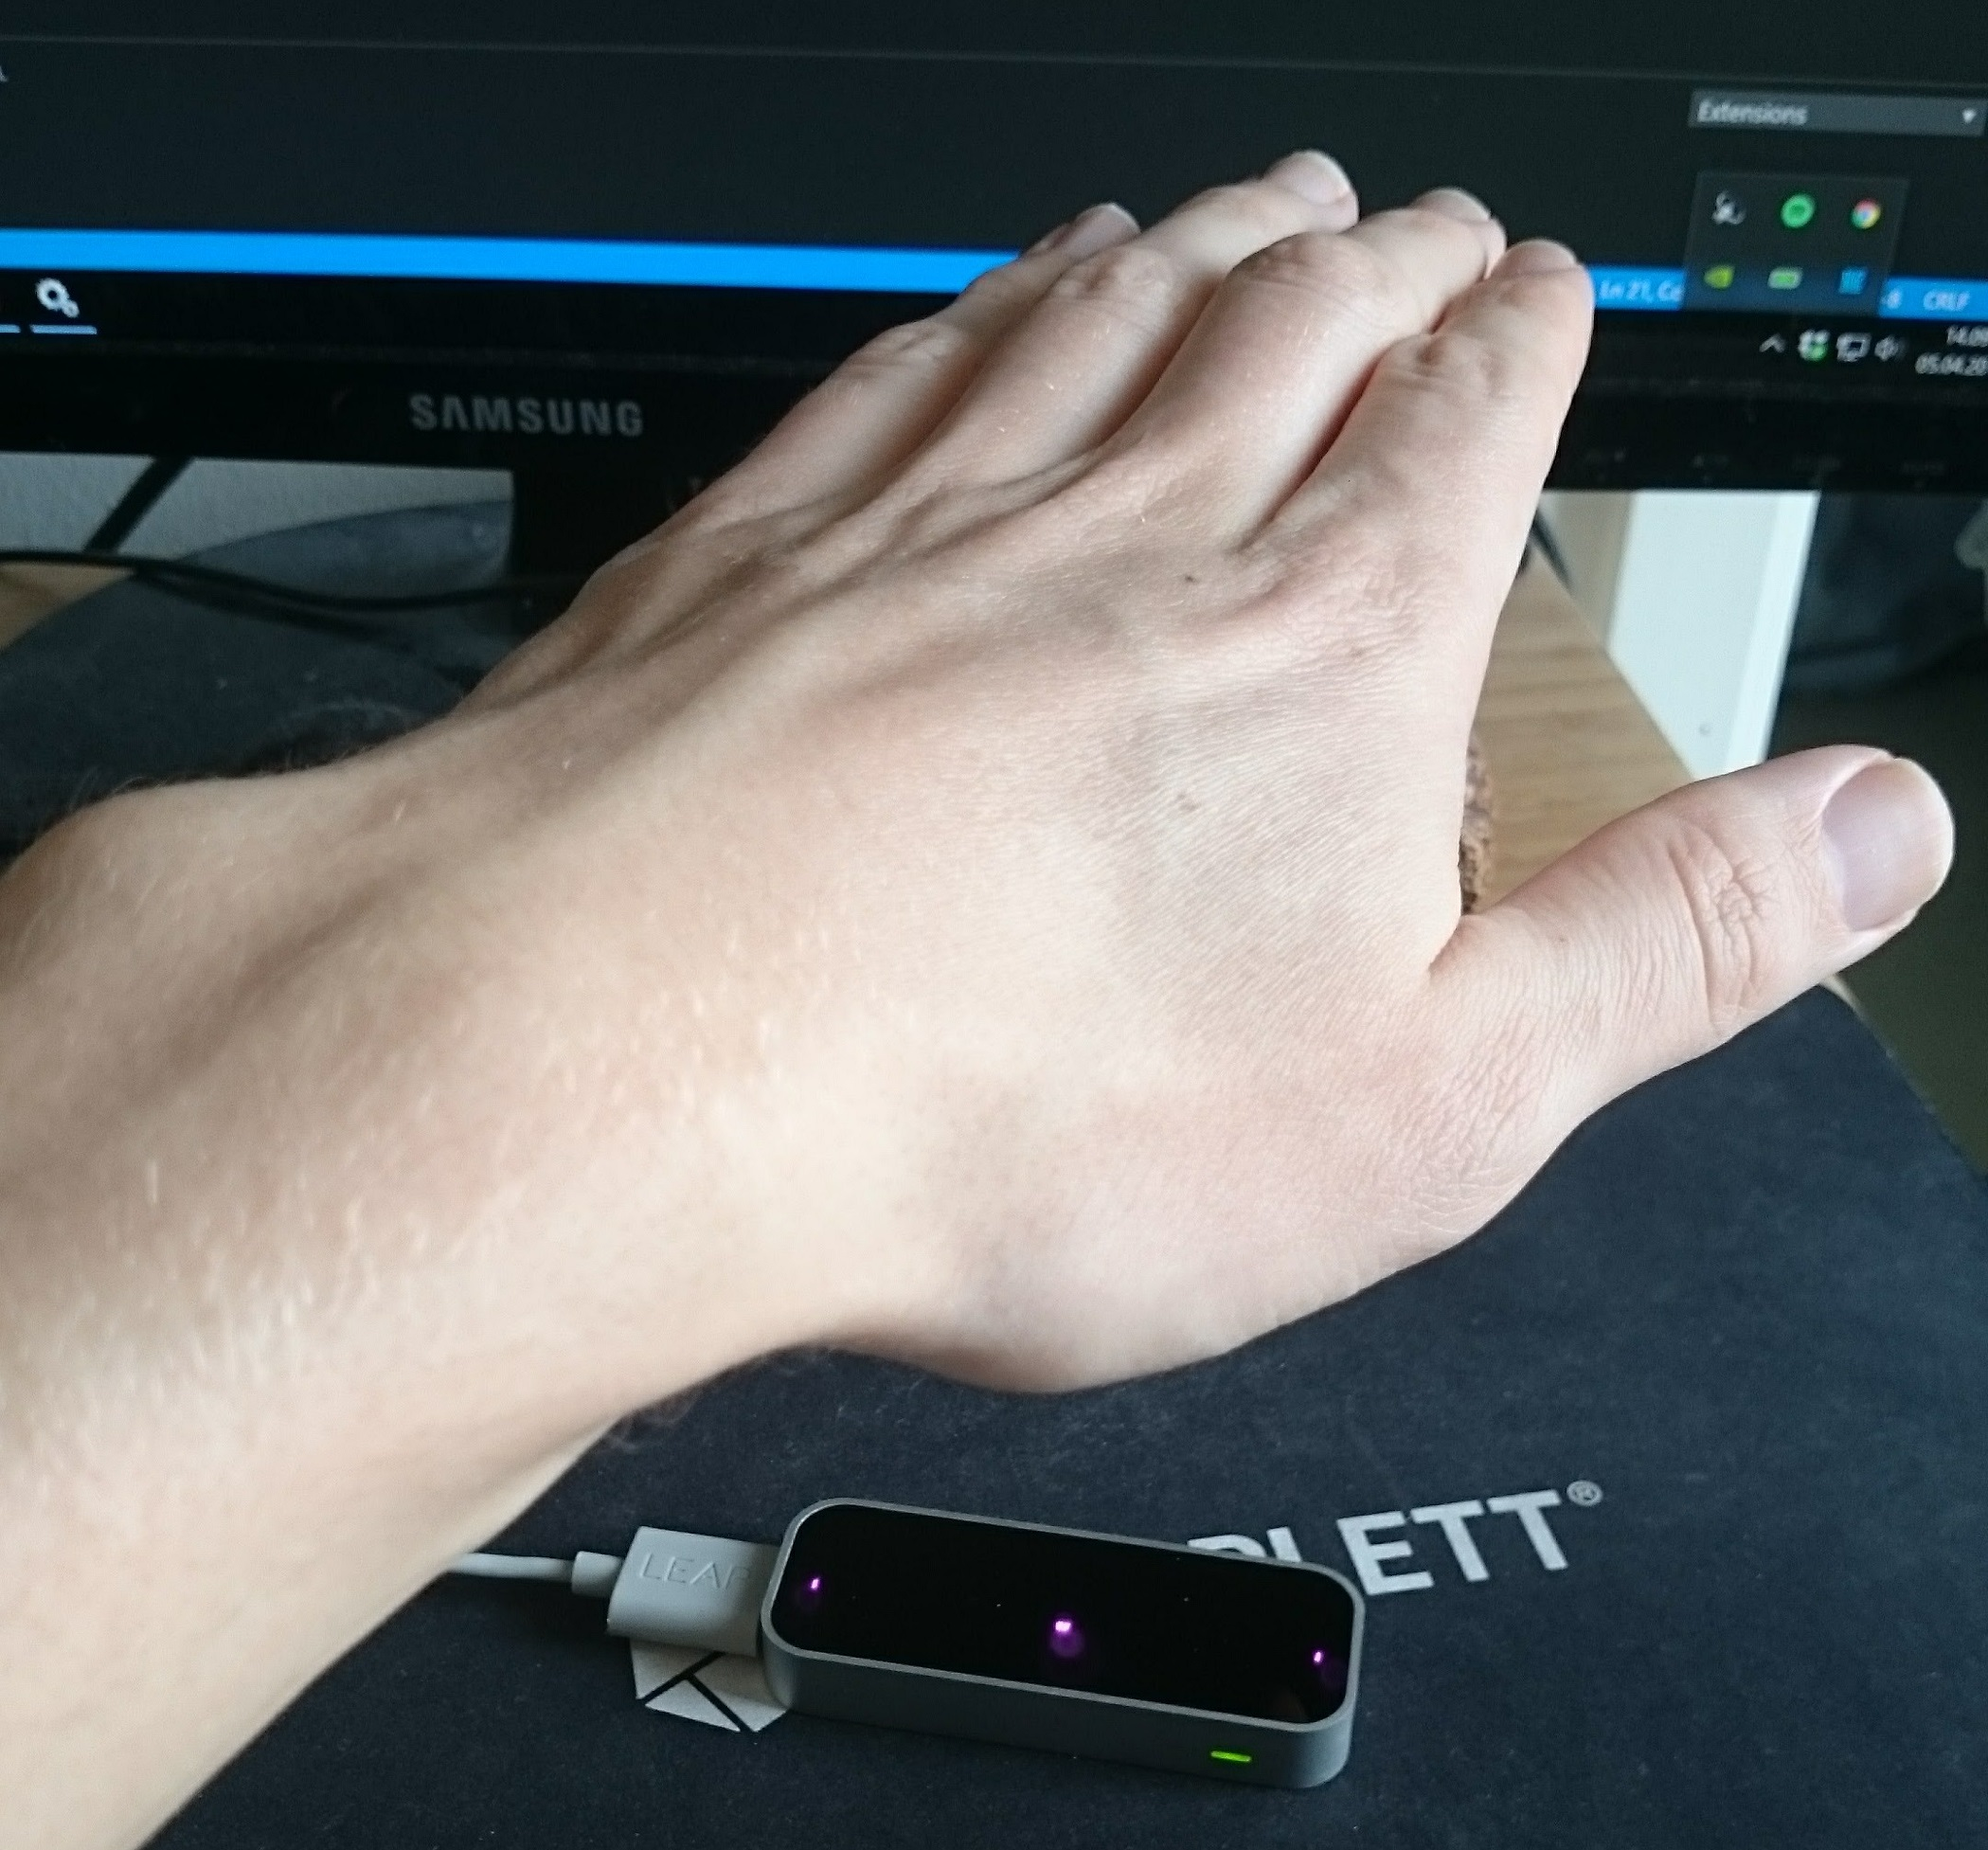
\includegraphics[width=0.5\linewidth]{pictures/gestures/palmdown.jpg}
	\caption[The pinch and palm-down gestures]{The pinch gesture (left) is used to rotate the camera along the y- and z-axis. 
             The palm-down gesture (right) is used to move the user up and down along the y-axis.}
	\label{fig:gestures1}
\end{figure} 

\subsection{The Palm-down Gesture}
\label{sec:palm_down_design}
The palm-down gesture, alternatively called the Y-gesture, fulfills the up-and-down functionality specified in the move use case, and enables the user to 
move along the y-axis, relative to its orientation. The palm-down gesture is accomplished simply by having all fingers extended, with all of them pointing in
the direction of the display with the palm facing downwards towards the table top (see~\vref{fig:gestures1} for an illustration). This gesture, along with the rest of the 
movement gestures (i.e the two following), uses the same origin-offset scheme as the pinch gesture, but the offset is in this gesture only measured on the y-axis, 
so moving the hand to the 
right, as mention in the pinch gesture section, will cause no movement when the palm-down gesture is the active gesture. 
Instead the user can move his or her hands up and down on the y-axis, so the distance to the table top increases or decreases.  

\subsection{The Palm-side Gesture}
The palm-side gesture, alternatively called the X-gesture, fulfills the left-and-right functionality specified in the move use case, and enables the user to 
move along the x-axis, relative to its orientation. The palm-side gesture is accomplished simply by having all fingers extended, with all of them pointing in
the direction of the display with the palm perpendicular (i.e~at a 90° or 270° angle) to the table top (see~\vref{fig:gestures2} for an illustration). 
As one of the movement gesture, this gesture also uses the origin-offset scheme, but only with the x-axis monitored.

\subsection{The Fist Gesture}
The fist gesture, alternatively called the Z-gesture, fulfills the forward-and-backwards functionality specified in the move use case, and enables the user to 
move along the z-axis, relative to its orientation. The fist gesture is accomplished by forming a fist (i.e with no fingers extended)
and is used by extending and retracting the fist. 

\begin{figure}%[h!] %[H]
	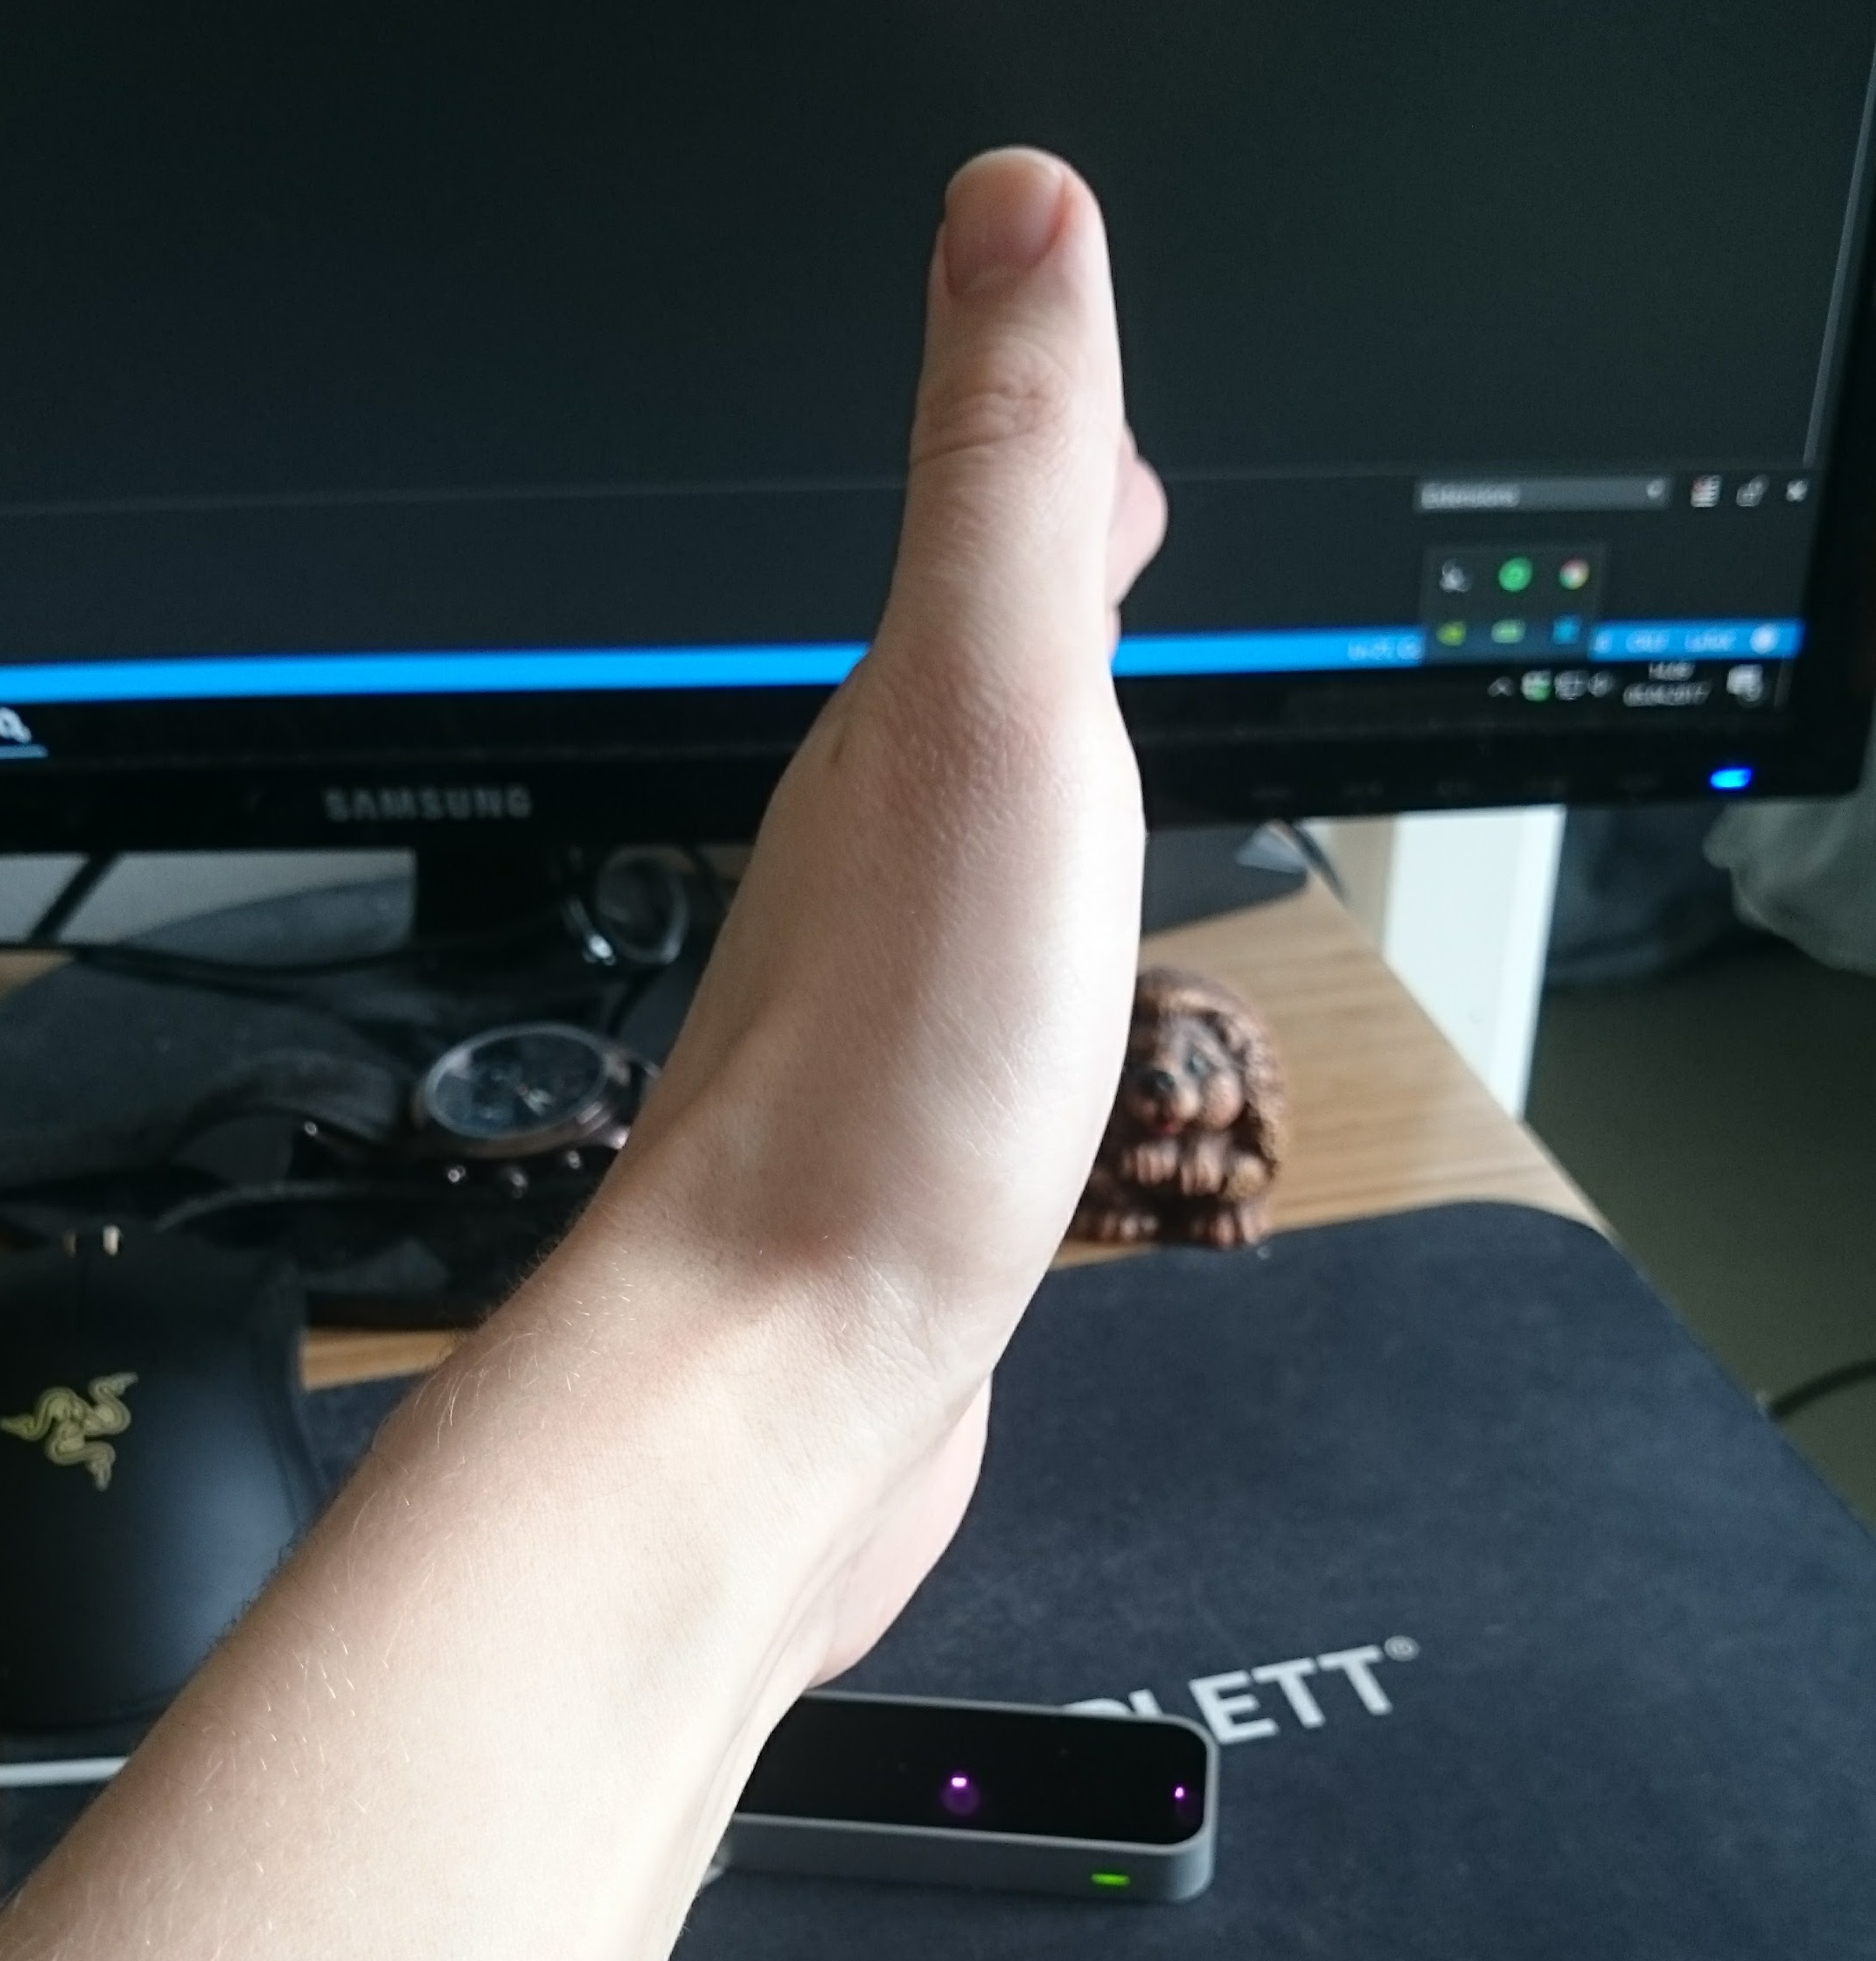
\includegraphics[width=0.5\linewidth]{pictures/gestures/palmside.jpg}
    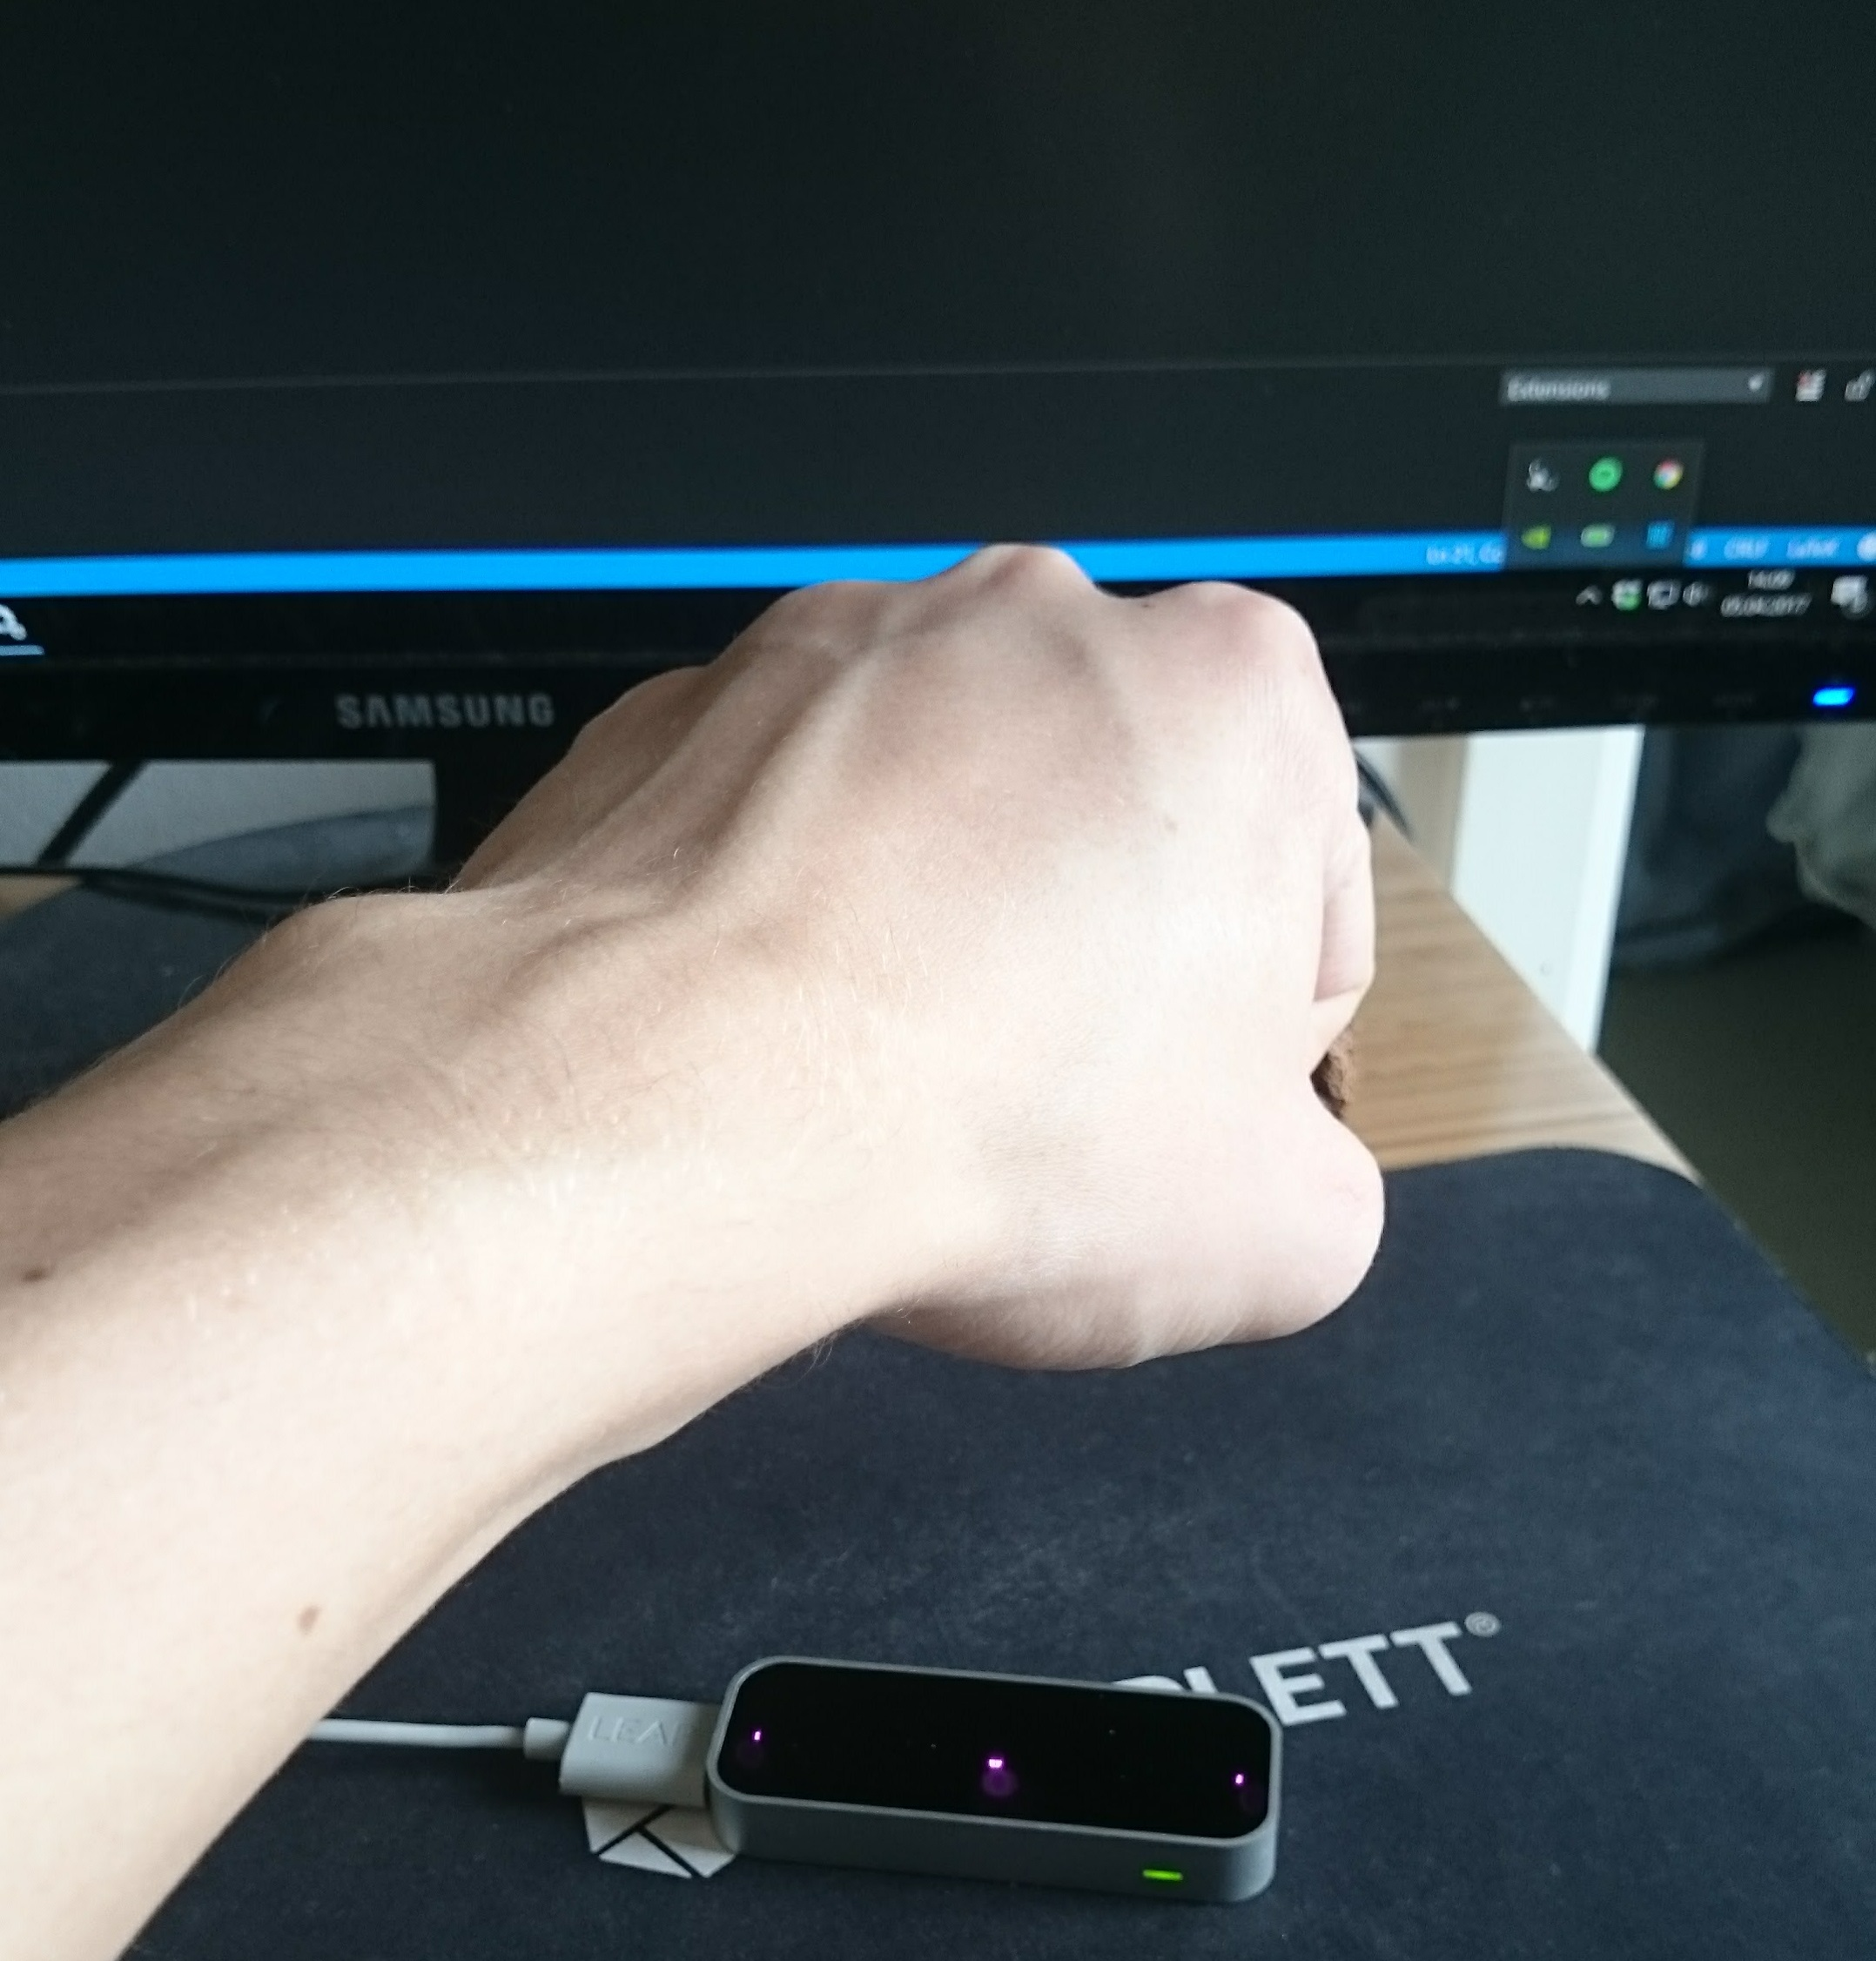
\includegraphics[width=0.5\linewidth]{pictures/gestures/fist.jpg}
	\caption[The palm-side and fist gestures]{The palm-side gesture (left) is used to move the user left and right along the x-axis. 
             The fist gesture (right) is used to move the user forward and backward along the z-axis.}
	\label{fig:gestures2}
\end{figure} 

\subsection{The Combined-movement Gesture}
\label{sec:combined-movement}
The combined-movement gesture, alternatively called the XYZ-gesture, is a special gesture that's only enabled if the "use combined gesture" option is selected in the menu.
When this option is enabled the other movement gestures, i.e the palm-down-, the palm-side- and the fist gesture, should be disabled and instead replaced by a combined version. 
When this is the case, the "use combined gesture" option should be replace by a "distinguish movement gestures" option in the menu, 
which disabled this combined gesture and re-enabled the default movement gestures. 

The combined movement gesture should be performed in the same manner as the palm-down gesture, described in section~\ref{sec:palm_down_design}, 
and can thus be considered an overload\footnote{A concept where the same identifier (a gesture in this case) can perform different actions based on a current state or context (i.e whether the combined gesture scheme is active or not.)}.
%i.e by having all fingers extended, with all of them pointing in the direction of the display with the palm facing downwards towards the table top.
However, instead of now only being responsible for navigation along the y-axis, i.e up and down, this same gesture is now responsible for movement along the x-, y- and z-axis, so
all hand movement (along all axes) is monitored and reflected as movement when the combined gesture is active.
The idea behind reusing a gesture is because it limits the number of unique gestures needed, and thus diminishes the possibility of two gestures being so similar 
that the gesture recognition system often confuses them. The palm-down gesture is selected because is arguably is one of the more ergonomic and comfortable gestures to perform. 
Also note that when the palm-down gesture is used in combined-gesture mode the origin-offset scheme is still used, but now all the three dimensions are monitored. 

\subsection{The Single-point Gesture}
The single-point gesture is used to annotate a point or edit a point annotation, and is used by having the index finger extended and "pointing" at the display while the 
rest of the fingers are non-extended (the thumb can be either extended or not extended). 
When the user does the single-point gesture, a raycast (a kind of invisible beam) should be fired from the user towards where the user is facing.
The player should thus be able to aim, e.g.~by utilizing a crosshair in the middle of the players screen, by looking at a spot and use the single-point gesture to fire off 
the raycast. At the point the raycast collides with a part of the model a point annotation should be created. If the user use the single-point gesture again, while
still aiming at the same spot (where an annotation now should be present), the annotation form should open up to allow the user to input annotation information. 

\subsection{The Double-point Gesture}
The double-point gesture is used to annotate an object by highlighting it, or to edit a object annotation. The double-point gesture is invoked by pointing the index- and
middle finger at the screen with a slight angle between them, while the rest of the fingers are non-extended (the thumb can be either extended or not extended).
Apart from this the double-point gesture function very similar to the point gesture, with some few exception. Object annotations are edited by using the 
double-point gesture at them again, as opposed to using the single-point gesture, which created a point annotation on the annotated and highlighted object.

\begin{figure}%[h!] %[H]
	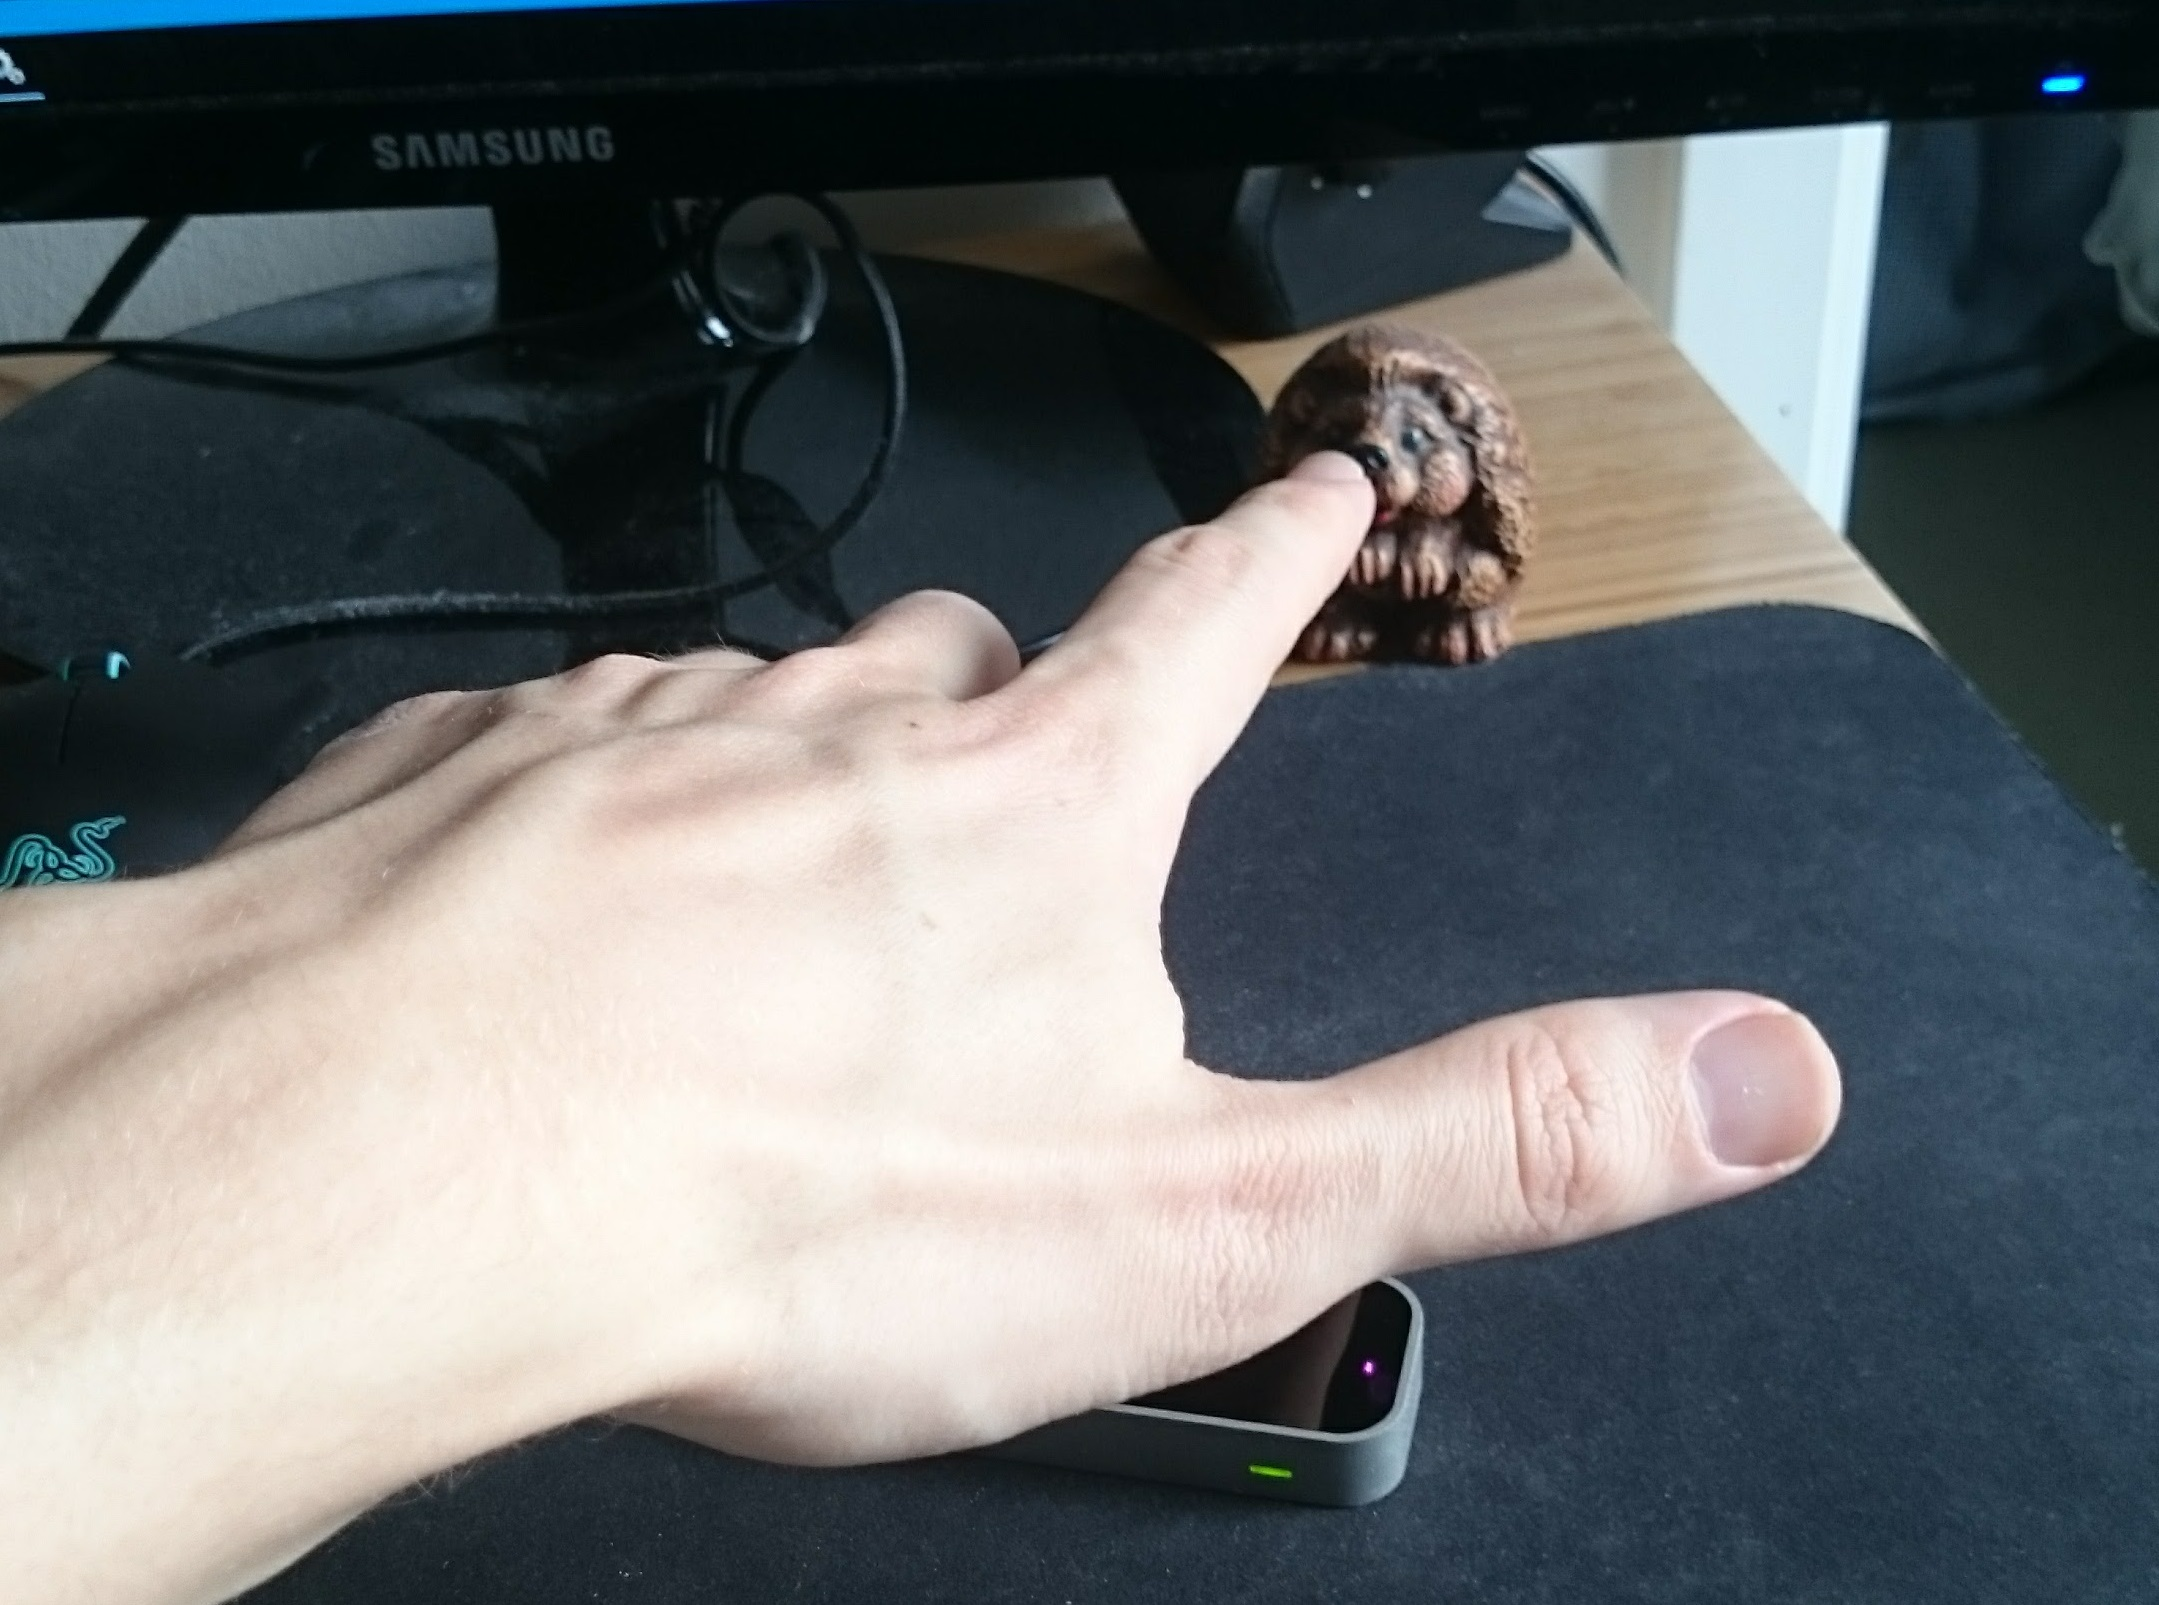
\includegraphics[width=0.5\linewidth]{pictures/gestures/singlepoint.jpg}
    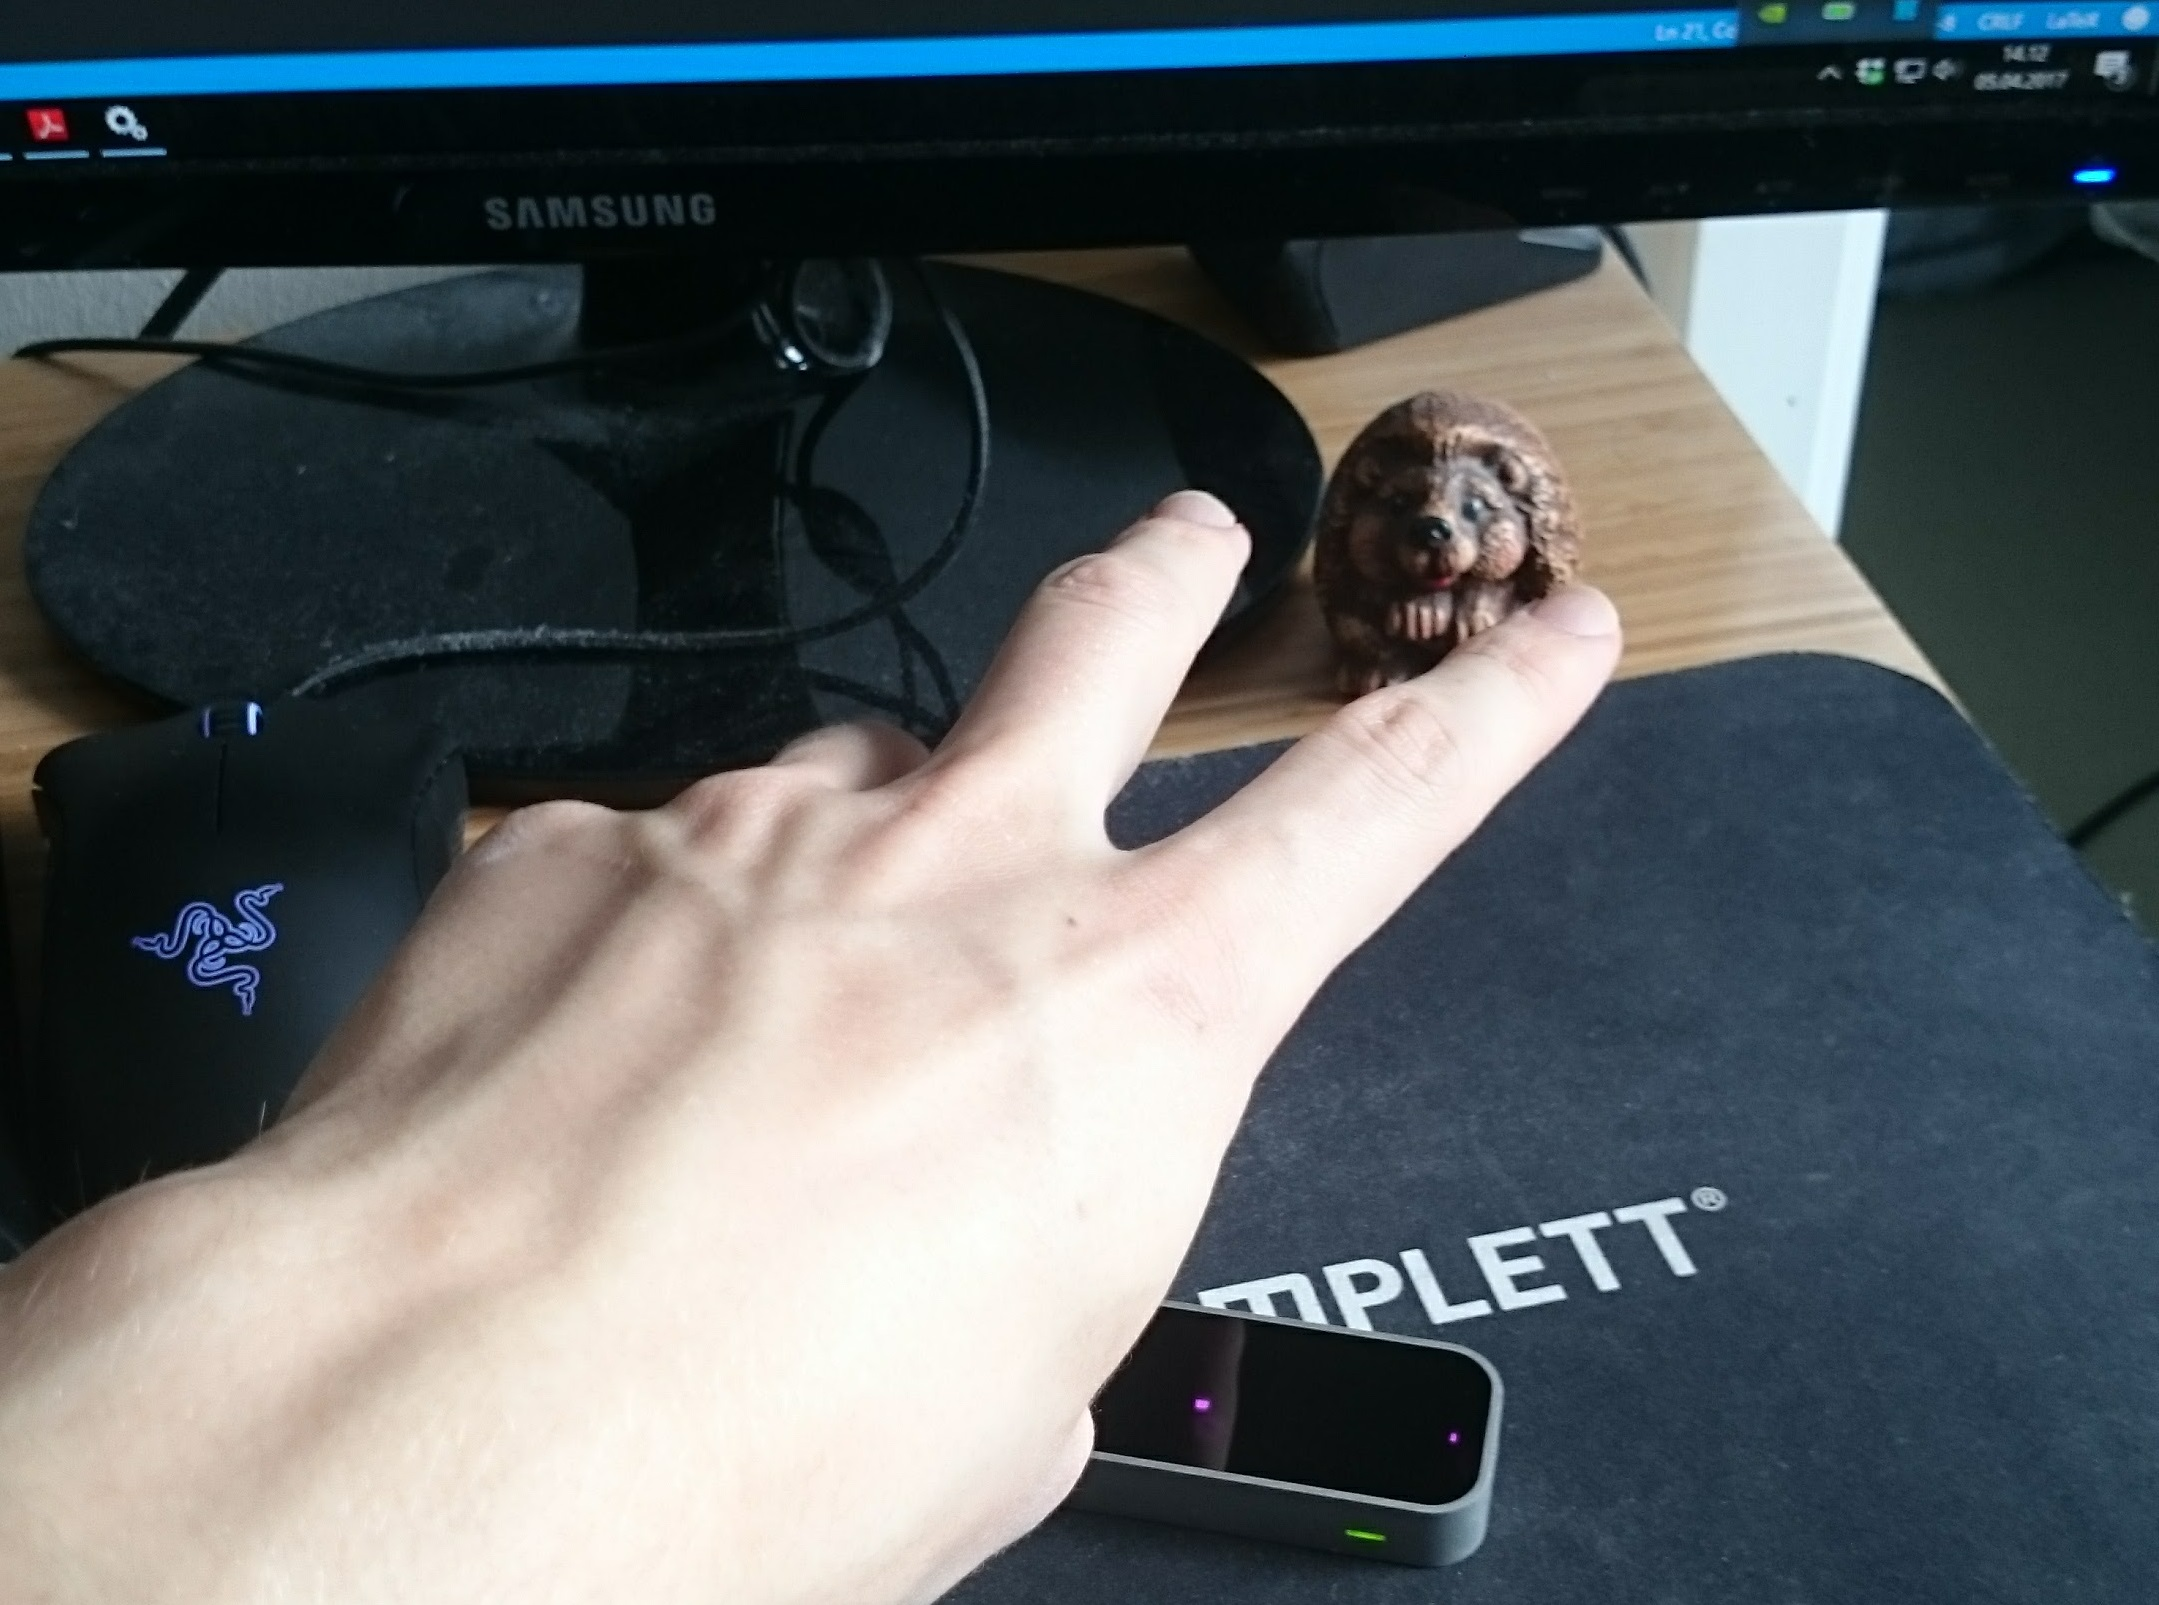
\includegraphics[width=0.5\linewidth]{pictures/gestures/doublepoint.jpg}
	\caption[The single-point and double-point gestures]{The single-point gesture (left) is used to create or edit a point annotation. 
             The double-point gesture (right) is used to create or edit an object annotation.}
	\label{fig:gestures3}
\end{figure} 

\subsection{The Menu Gesture}
The menu gesture gives the user access to a menu especially design to use with gestures. The menu is invoked by extending all fingers on 
"the menu hand" (the left hand by default) and turn it so the palm faces the user. When this gesture is recognized by the system a menu should 
appear in the shape of a fan with its root in the palm of the user. The user can then use the index finger on the other hand, "the selector hand" (right hand by default),
and click on one of the buttons by holder the tip of the index finger within the range of the button (i.e close enough to the button in terms of x-, y- and z coordinates).
If the tip of the index finger is close enough to the button, the button will start to "fill up", indicating that it is in the process of being pressed.
Once the button is "filled up" the selection is registered and the action the button represents is carried out. Not that this mechanism is in place
to prevent miss-clicks from the user.
